\subsection{Introduction}

\begin{figure*}
    \centering
    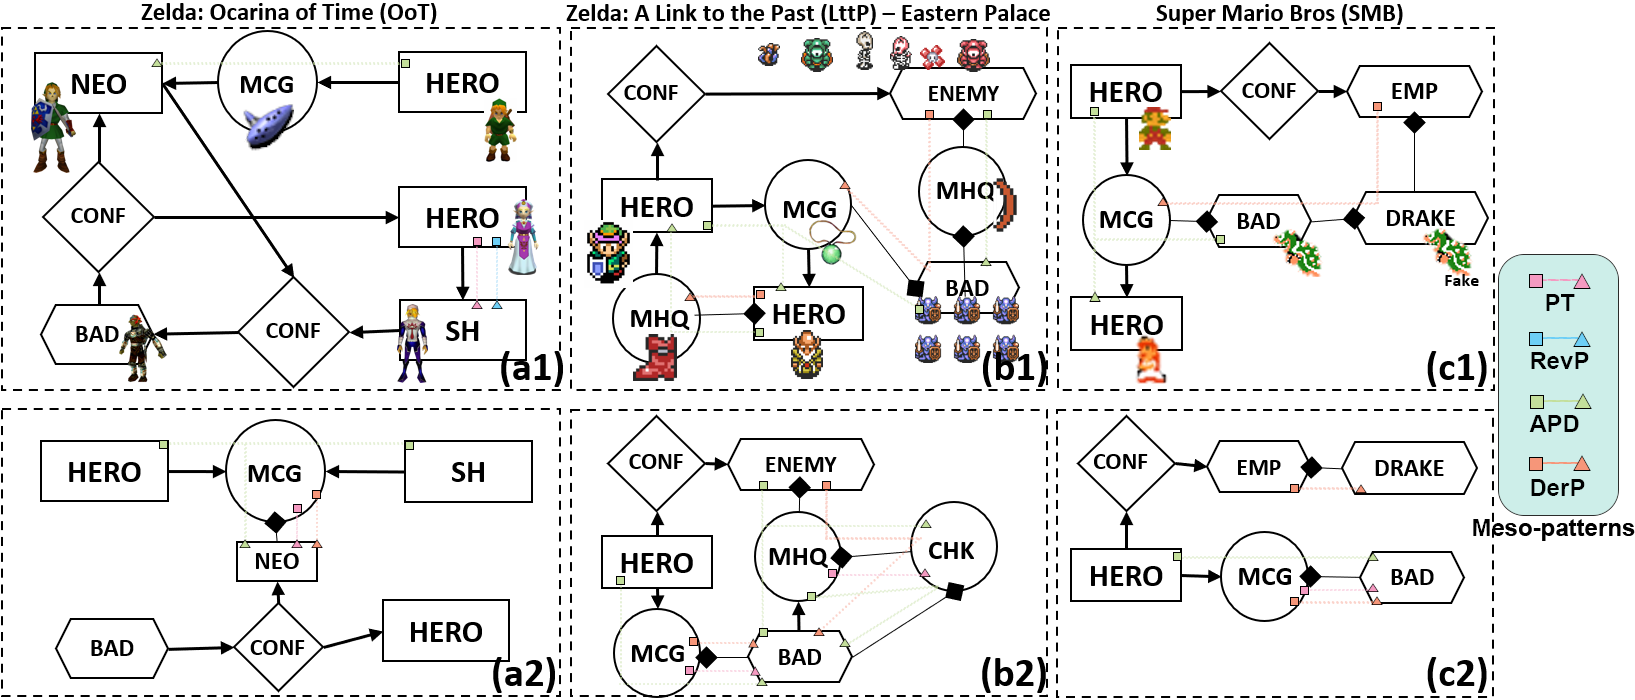
\includegraphics[width=0.95\textwidth]{figures/figure-1_extra8.png}
       \caption{Proof-of-concept narrative structures of existing games (top row) created using TropeTwist with the available nodes (table~\ref{tab:tropes}). Bottom row shows exemplar elites generated with MAP-Elites using the respective top row narrative structure as root. Color matching squares, lines, and triangles denote different meso-patterns in the structures. Squares and triangles are the start and end of a meso-pattern, respectively.}
       \label{fig:teaserfig}
\end{figure*}

There exists a plethora of games\footnote{For instance, currently there are more than 68k games in steam \url{https://store.steampowered.com/search/?category1=998}.}, with diverse genres and each containing a different set of gameplay mechanics, audio, level, graphic, and narrative facets. The creation and combination of these facets make game development a hard task, commonly involving a diverse group of developers~\cite{p12Blow2004-gamesHard}. Likewise, the generation of these facets in conjunction has been categorized as one of the biggest and most challenging tasks within computational creativity~\cite{p12Liapis2014-gameCreativity,Liapis2019-OrchestratingGames}. However, games share common elements and underlying narratives, but it is non-trivial how to identify these, how to define and analyze these games structurally, or what type of common underlying structures exist; pointed out as well by~\cite{p12aarseth2018-ontologicalMeta,vozaru_game_2022}.

Among the different facets, narrative stands out in games as it helps to create meaning, make sense of situations, and make games [stories] recognizable~\cite{p12mateas2003-facade,Aarseth2012-Narrativetheory,kybartas2016survey,flodtol2020-WIPMakeSenseDungs}. Narrative structures can be used to describe how an experience or story is to be developed as argued by Barthes~\cite{p12Barthes75-introStructNarr}, and to create an abstract representation based on the narrative structure instead of a temporal and partially-ordered sequence of events~\cite{p12Szilas2003-structuralModelsIDtension}. Common narrative structures used in many domains are Aristotle's drama structure, which subdivides a story into \textit{exposition}, \textit{climax}, and \textit{resolution} or Propp's analysis on the morphology of russian folktale, which revealed a common structure among them, denoted as Propp's 31 ``narremes''~\cite{p12propp1975-morphology}.

This paper presents \emph{TropeTwist}, a preliminar system that uses Tropes~\cite{p12Thompson2018-usingTropesNarrativeEvents,tropesSimpsons} extracted from TvTropes~\cite{p12tvtropes,periodicTable} as patterns and fundamental units, which when combined can compose structures further representing other composed tropes. Common narrative structures can be identified and defined using \emph{TropeTwist}. TropeTwist can define generic aspects of a story, leading to the identification of events, roles, and narrative elements, as well as a novel way to form narratives. As a proof-of-concept, we built, analyzed, and described structurally three game examples shown in figure~\ref{fig:teaserfig}, top row.

%We propose graph grammars as indirect encoding of narrative graphs and the use of the Multi-dimensional Archive of Phenotypic Elites (MAP-Elites)~\cite{p12Mouret2015-MAPElites} to generate novel variations (shown in figure~\ref{fig:teaserfig}, bottom row) using the proof-of-concept examples as roots. Simultaneously, we propose metrics to evaluate the coherence, cohesion, and interestingness of the resulting narrative graphs, which we use as comparison between hand-made and generated narrative graphs. Our preliminary results show that by using MAP-Elites, it is possible to vary the structure in such a way that more interesting structures appear while retaining coherence. 

We propose graph grammars as indirect encoding of narrative graphs and the use of the Multi-dimensional Archive of Phenotypic Elites (MAP-Elites)~\cite{p12Mouret2015-MAPElites} to generate novel variations (shown in figure~\ref{fig:teaserfig}, bottom row) using the proof-of-concept examples as roots. Simultaneously, we propose metrics to evaluate the resulting narrative graphs' coherence, cohesion, and interestingness. Our preliminary results show that we can produce more interesting structures retaining coherence based on our metrics. 

% We propose indirectly encoding these as graph grammars and using the Multi-dimensional Archive of Phenotypic Elites (MAP-Elites)~\cite{p12Mouret2015-MAPElites} to generate 

% We Further, using graph grammars and evolutionary algorithms (EA) and these graphs as targets and roots, we show preliminary results on how to generate and evaluate novel variations using the Multi-dimensional Archive of Phenotypic Elites (MAP-Elites)~\cite{p12Mouret2015-MAPElites}. We evaluate the proof-of-concept narrative graphs and the generated ones based on their inter



% In our system, narrative structures serve as an abstraction layer, which can be used to create more generic aspects of a story, and at the same time, we can leverage its ambiguity as the structure is not necessarily bounded to specific partially-ordered events. As a proof-of-concept, we built, analyzed, and described structurally three game examples shown in figure~\ref{fig:teaserfig}, top row. Further, using graph grammars and evolutionary algorithms (EA) and these graphs as targets and roots, we show preliminary results on how to generate and evaluate novel variations using the Multi-dimensional Archive of Phenotypic Elites (MAP-Elites)~\cite{p12Mouret2015-MAPElites}. We evaluate the proof-of-concept narrative graphs and the generated ones based on their inter

% This could allow a designer to create the structure of what they intend the narrative to be rather than focusing on how it will occur, how to communicate it to the player, or the specific plot points. As a proof-of-concept, we built, analyzed, and described structurally three game examples shown in figure~\ref{fig:teaserfig}, top row. Further, using graph grammars and evolutionary algorithms (EA) and these graphs as targets and roots, we show preliminary results on how to generate and evaluate novel variations.

% In our system, narrative structures serve as an abstraction layer, which can be used to create more generic aspects of a story, and at the same time, we can leverage its ambiguity as the structure is not necessarily bounded to specific partially-ordered events. This could allow a designer to create the structure of what they intend the narrative to be rather than focusing on how it will occur (i.e., syuzhet), how to communicate it to the player (i.e., discourse), or the specific plot points (i.e., fabula). As a proof-of-concept, we built, analyzed, and described structurally three game examples shown in figure~\ref{fig:teaserfig}, top row. Further, using graph grammars and evolutionary algorithms (EA) and these graphs as targets and roots, we show preliminary results on how to generate and evaluate novel variations.